% IEEE Conference template (IEEEtran)
% Suitable for CVPR, ICCV, ICRA, INFOCOM and most IEEE-style venues.
\documentclass[conference]{IEEEtran}
\IEEEoverridecommandlockouts

\usepackage[a4paper,margin=25mm]{geometry}
\usepackage{cite}
\usepackage{graphicx}
\usepackage{booktabs}
\usepackage{array}
\usepackage{longtable}
\usepackage{amsmath,amssymb,amsfonts}
\usepackage{algorithmic}
\usepackage{xcolor}
\usepackage{hyperref}
\usepackage{caption}
\usepackage{float}
\usepackage{enumitem}

\hypersetup{
    colorlinks=true,
    linkcolor=black,
    citecolor=blue,
    urlcolor=blue,
}
\sloppy
\emergencystretch=2em
\allowdisplaybreaks

\begin{document}

\title{From PEFT to DEFT: Parameter Efficient Finetuning for Reducing Activation Density in Transformers}

\author{
\IEEEauthorblockN{Bharat Runwal \(^{1}\)} \and \IEEEauthorblockN{Tejaswini Pedapati \(^{2}\)} \and \IEEEauthorblockN{Pin-Yu Chen \(^{2}\)}}

\maketitle

\begin{abstract}
Pretrained Language Models (PLMs) serve as the foundational framework for fine-tuning in downstream tasks. However, the growing scale of these models presents challenges for traditional fine-tuning approaches that update all parameters. To mitigate this, parameter-efficient fine-tuning (PEFT) methods have emerged as a viable solution for adapting PLMs effectively. Concurrently, recent research has identified activation sparsity in the intermediate outputs of multilayer perceptron (MLP) blocks within transformer architectures. This sparsity enables efficient model inference on hardware optimized for sparse computations. In this work, we introduce a novel \textbf{density loss} function designed to promote higher activation sparsity (i.e., lower activation density) in pretrained models. Our proposed method, \textbf{DEFT (Density-Efficient Fine-Tuning)}, leverages mainstream PEFT techniques—including QLoRA, LoRA, Adapter, and Prompt/Prefix Tuning—to enhance model adaptation across diverse downstream tasks. Empirical evaluations demonstrate that DEFT achieves substantial reductions in activation density: up to \textbf{44.94\%} on RoBERTa\(_{Large}\) and \textbf{53.19\%} (encoder) and \textbf{90.60\%} (decoder) on Flan-T5\(_{XXL}\) (11B) compared to standard PEFT, as measured on GLUE and QA (SQuAD) benchmarks, while maintaining competitive task performance. Furthermore, we present \textbf{ADA-DEFT}, an adaptive variant of DEFT that optimizes inference efficiency. ADA-DEFT yields notable improvements in computational resource utilization, reducing runtime by \textbf{8.75\%} and memory consumption by \textbf{16.78\%} for Flan-T5\(_{XL}\), and by \textbf{2.79\%} and \textbf{2.54\%}, respectively, for Flan-T5\(_{XXL}\). Our results also indicate that DEFT operates synergistically with quantized and pruned models, further enhancing their efficiency. \textbf{Code Availability:} https://github.com/IBM/DEFT
\end{abstract}


\section{Introduction}

The emergence of pre-trained large language models (LLMs) (Devlin et al., 2019; Radford et al., 2019; Raffel et al., 2020) has popularized fine-tuning as a standard approach for task adaptation (Howard \& Ruder, 2018). However, the computational demands of training and inference for these models entail substantial time, energy, and memory consumption, contributing to a significant carbon footprint (Strubell, Ganesh, \& McCallum, 2019). To address these challenges, researchers have explored various methods for efficient inference, including parameter pruning (Lee, Ajanthan, \& Torr, 2019; Tanaka et al., 2020), attention head reduction through pattern analysis (Behnke \& Heafield, 2020; Voita et al., 2019; Michel, Levy, \& Neubig, 2019), model distillation (Sanh et al., 2019), weight quantization (Dettmers et al., 2022; Zadeh et al., 2020), and mixture-of-experts architectures (Kudugunta et al., 2021; Rajbhandari et al., 2022). In contrast, this work focuses on accelerating inference by increasing activation sparsity in transformer models through a novel density-aware loss function. Recent studies (Zhang et al., 2021; Li et al., 2022) have demonstrated that transformer architectures exhibit sparse activation patterns, particularly in the intermediate outputs of Multi-Layer Perceptron (MLP) blocks with ReLU activations, where only a fraction of neurons activate for a given input. Building on this observation, we introduce a density loss function that explicitly encourages higher activation sparsity during fine-tuning, thereby reducing the density of non-zero activations. This approach not only enhances computational efficiency but also aligns with the capabilities of modern hardware accelerators, such as Application-Specific Integrated Circuits (ASICs) (Lazzaro et al., 2023), which exploit zero-skip operations to bypass computations involving zero-valued activations. By optimizing activation sparsity, our method enables energy-efficient inference, making it particularly suitable for resource-constrained environments. We propose Density-Efficient Fine-Tuning (DEFT) and its adaptive variant, ADA-DEFT, which integrate activation sparsity with parameter-efficient fine-tuning (PEFT) techniques. As illustrated in Figure 1a, DEFT achieves a marked reduction in activation density—defined as the average proportion of non-zero values in MLP layer outputs across the validation set—compared to standard PEFT. Furthermore, Figure 1b demonstrates the runtime savings of ADA-DEFT, where MLP blocks are dynamically skipped during inference based on learned layerwise weights, as evaluated on Flan-T5 models. To our knowledge, this work is the first to demonstrate that substantial activation sparsity can be achieved with minimal trainable parameters, even in models employing Gaussian Error Linear Unit (GeLU) activations (Hendrycks \& Gimpel, 2016), the default choice in state-of-the-art transformers. Prior research on activation sparsity has predominantly focused on ReLU-based models (Lazzaro et al., 2023), which inherently exhibit sparser activations. By combining PEFT with sparsity optimization, our approach advances the development of resource-efficient transformer models for diverse applications.


\begin{figure}[!t]
    \centering
    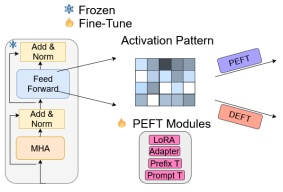
\includegraphics[width=\columnwidth]{figures/remote_377ec90f22d9.jpg}
    \caption{Image}
    \label{fig:1}
\end{figure}
\begin{figure}[!t]
    \centering
    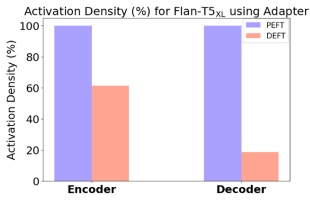
\includegraphics[width=\columnwidth]{figures/remote_cec287cbcc5e.jpg}
    \caption{Image}
    \label{fig:2}
\end{figure}
\begin{figure}[!t]
    \centering
    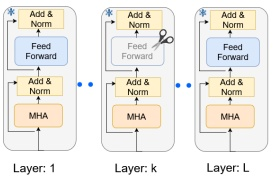
\includegraphics[width=\columnwidth]{figures/remote_f0ec24b0af5c.jpg}
    \caption{Image}
    \label{fig:3}
\end{figure}
\begin{figure}[!t]
    \centering
    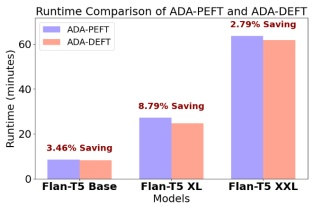
\includegraphics[width=\columnwidth]{figures/remote_74838162bcb1.jpg}
    \caption{Image}
    \label{fig:4}
\end{figure}


\section{Related Work}




\section{Weight Induced Sparsity}

\subsubsection*{Weight-Induced Sparsity}
Reducing the number of model parameters decreases the model's memory footprint and lowers the computational resources required for inference. This can be achieved through pruning, a technique that selectively removes parameters whose absence does not significantly degrade model performance. Unstructured pruning methods, such as SNIP (Lee, Ajanthan, \& Torr, 2019), GraSP (Wang, Zhang, \& Grosse, 2020), and Synaptic Flow (Tanaka et al., 2020), enable weight pruning at initialization. Prior work has explored structured pruning by ranking attention heads or weights based on importance metrics. For example, Michel, Levy, and Neubig (2019) compute importance scores as the difference in loss values when a head is retained versus pruned. Similarly, Voita et al. (2019) and Behnke and Heafield (2020) employ head confidence as a pruning criterion. An alternative approach involves distilling a large model into a smaller, parameter-efficient version. DistilBERT (Sanh et al., 2019), for instance, was derived from BERT via knowledge distillation during pre-training, achieving a 40\% reduction in size while retaining 97\% of BERT’s performance. Chen et al. (2021) introduced a parameter-efficient fine-tuning method that applies low-rank weight updates akin to LoRA. This approach allows users to specify desired sparsity levels and choose whether to prune entire heads or individual parameters. Post-training, parameters and heads are ranked by gradient magnitude and pruned according to user preferences to meet the target sparsity. Sun et al. (2023a) further refine pruning by defining importance scores as the product of weight magnitudes and input activation norms, ensuring a principled selection of parameters for removal.




\section{Activation Induced Sparsity}

\textbf{Activation-Induced Sparsity} Unlike static parameter pruning, activation-induced sparsity dynamically reduces computational latency by selectively suppressing neural activations during inference, leveraging sparsity-aware hardware acceleration. Empirical studies by Li et al. (2022) demonstrate that larger language models exhibit progressively sparser layer outputs, though no neuron remains entirely inactive. Specifically, while 93.5\% of neurons were activated fewer than 10\% of the time, even the least active neuron exhibited a non-zero firing rate of at least 0.001\%. This sparsity is achieved by thresholding the top-k activations and zeroing out all others. In a related approach, Kurtz et al. (2020) introduced a modified ReLU activation for ResNet18 models, where neurons fire only if their input magnitude exceeds a predefined threshold, coupled with a specialized sparsity-aware convolution algorithm to optimize inference. In contrast, our method inherently induces activation sparsity during training through a carefully designed loss function, eliminating the need for post hoc architectural modifications.




\section{Methodology}




\section{Background and Notations}

In transformer architectures, position-wise feed-forward networks typically consist of a two-layer multilayer perceptron (MLP). To analyze activation sparsity, we focus on the intermediate output of this MLP, building upon methodologies established by Li et al. (2022) and Zhang et al. (2021). Let \(X \in \mathbb{R}^{B \times K \times d_{\text{model}}}\) denote an input tensor, where \(B\) represents the batch size, \(K\) the sequence length, and \(d_{\text{model}}\) the dimensionality of input features. The output of the two-layer MLP is given by: \[Y(X; W_1, W_2) = f(X W_1) W_2,\] where \(W_1 \in \mathbb{R}^{d_{\text{model}} \times d_{\text{ff}}}\) and \(W_2 \in \mathbb{R}^{d_{\text{ff}} \times d_{\text{model}}}\) are learnable weight matrices, \(d_{\text{ff}}\) is the hidden dimension of the MLP, and \(f\) denotes a non-linear activation function.
\subsubsection*{Gated MLP Blocks}
Modern large language models (LLMs) predominantly employ gated MLP blocks (Shazeer, 2020), which introduce a gating mechanism defined as: \[Y = \left( f(X W_s^T) \odot (X W_e^T) \right) W_o^T,\] where \(W_s, W_e \in \mathbb{R}^{d_{\text{ff}} \times d_{\text{model}}}\) and \(W_o \in \mathbb{R}^{d_{\text{model}} \times d_{\text{ff}}}\) are learnable parameters.
\subsubsection*{Activation Sparsity Measurement}
To quantify activation sparsity, we first compute the activation pattern \(O\), defined as: \[O = f(X W_1) \quad \text{or} \quad O = f(X W_s^T).\] Here, \(O \in \mathbb{R}^{B \times K \times d_{\text{ff}}}\) captures the activation states across batches and sequence positions. Following Li et al. (2022), we derive a feature map \(s \in \mathbb{R}^{d_{\text{ff}}}\) by averaging \(O\) over batches and sequence lengths. The sparsity of neuron activations is then measured by counting the non-zero entries in \(s\).




\section{Density Loss}

In this section, we present the Density loss component of DEFT, designed to reduce activation density (or equivalently, increase activation sparsity) in multilayer perceptron (MLP) blocks for given inputs. Prior work by Li et al. (2022) employed a step function to precisely count the number of positive activations. However, this approach is non-differentiable and thus incompatible with end-to-end learning frameworks. To address this limitation, we adopt a differentiable approximation for the number of non-zero entries in the sparse activation vector \textbf{s}. For ReLU-based models, we utilize a scaled hyperbolic tangent function (Equation 4) with parameter \(\beta\), applied to an input feature \textbf{x} comprising \(n\) elements \(\{x_{i}\}_{i=1}^{n}\). A similar approximation was previously used by Krithivasan et al. (2020) for generating adversarial inputs in sparsity attacks. For models employing activations other than ReLU (e.g., GeLU), we employ a differentiable \(l_{0}\)-norm approximation (Equation 5) with hyperparameter \(\epsilon > 0\), as proposed by Lazzaro et al. (2023). \textbackslash{}[ \textbackslash{}tanh(x, \textbackslash{}beta) = \textbackslash{}frac\{e\textasciicircum{}\{\textbackslash{}beta \textbackslash{}cdot x\} - e\textasciicircum{}\{-\textbackslash{}beta \textbackslash{}cdot x\}\}\{e\textasciicircum{}\{\textbackslash{}beta \textbackslash{}cdot x\} + e\textasciicircum{}\{-\textbackslash{}beta \textbackslash{}cdot x\}\} \textbackslash{}quad \textbackslash{}text\{(4)\} \textbackslash{}] \textbackslash{}[ \textbackslash{}hat\{l\}\textit{\{0\}(x, \textbackslash{}epsilon) = \textbackslash{}sum}\{i=1\}\textasciicircum{}\{n\} \textbackslash{}left( \textbackslash{}frac\{x\textit{\{i\}\textasciicircum{}\{2\}\}\{x}\{i\}\textasciicircum{}\{2\} + \textbackslash{}epsilon\} \textbackslash{}right) \textbackslash{}quad \textbackslash{}text\{(5)\} \textbackslash{}] The parameter \(\beta\) in Equation 4 controls the abruptness of the approximation, with higher values yielding a closer resemblance to the step function and thus promoting sparsity. In Equation 5, \(\epsilon \in \mathbb{R}\) governs the fidelity of the \(l_{0}\)-norm approximation, where smaller values yield more precise estimates. Additional approximation functions, including sigmoid and \(l_{1}\)-norm variants, are explored in Appendix A.3. The Density loss \(\mathcal{L}_{\text{density}}(x)\) is formally defined as: \textbackslash{}[ \textbackslash{}mathcal\{L\}\textit{\{\textbackslash{}text\{density\}\}(x) = \textbackslash{}frac\{1\}\{n\} \textbackslash{}sum}\{l=1\}\textasciicircum{}\{L\} \textbackslash{}sum\textit{\{i\} g(s}\{l\_\{i\}\}) \textbackslash{}] Here, \(n\) denotes the total number of neurons across all MLP layers, \(L\) is the number of transformer layers, and \(s_{l}\) represents the feature map following the first dense layer in the \(l\)-th MLP block, indexed by \(i\). The summation aggregates contributions from all layers and activation features. The function \(g\) may be instantiated as the \(l_{0}\)-norm approximation (Equation 5) or any alternative differentiable approximation discussed in Appendix A.3.




\section{Parameter Efficient Fine-tuning (PEFT)}

Fine-tuning large language models (LLMs) traditionally involves updating all model parameters, which incurs substantial computational costs. This approach becomes particularly inefficient when adapting a single model to multiple downstream tasks, as it requires storing a separate set of trained parameters for each dataset, resulting in significant storage overhead and computational redundancy. To mitigate these challenges, Parameter Efficient Fine-tuning (PEFT) introduces a limited set of additional trainable parameters while keeping the majority of the model frozen. By updating only these newly introduced parameters during fine-tuning, PEFT substantially reduces computational demands and storage requirements, as only the task-specific parameters need to be saved. This optimization streamlines the adaptation process without compromising model performance. The proposed DEFT framework is fully compatible with PEFT and incorporates several established techniques for demonstration, including Prompt Tuning (Lester et al., 2021), Prefix Tuning (Li \& Liang, 2021), Adapters (Houlsby et al., 2019), and Low-Rank Adaptation (LoRA) (Hu et al., 2022; Dettmers et al., 2023). A detailed discussion of each technique is provided in Appendix A.1.




\section{DEFT: Parameter and Activation Density Efficient Fine-tuning}

space{1em} \hrule space{1em}
\subsubsection*{DEFT: Parameter and Activation Density Efficient Fine-Tuning}
The DEFT framework enables efficient model adaptation by freezing the original transformer parameters and fine-tuning only the introduced parameter-efficient fine-tuning (PEFT) modules for downstream tasks. The optimization objective is formulated as:
\[\arg\min_{\Phi} \mathcal{L}_{T}\left(\mathbf{D}; \{\Theta, \Phi\}\right)\]
where \(\Phi\) denotes the trainable PEFT parameters and \(\Theta\) represents the frozen pre-trained model parameters. \(\mathcal{L}_{T}\) is the task-specific loss function evaluated on dataset \(\mathbf{D}\). To achieve activation sparsity in the MLP layers of transformer blocks, we extend the optimization problem by incorporating a density loss term:
\[\begin{aligned}
\arg\min_{\Phi} \mathcal{L}_{total} &= \mathcal{L}_{T}\left(\mathbf{D}; \{\Theta, \Phi\}\right) \\
&\quad + \alpha \cdot \mathcal{L}_{density}\left(\mathbf{D}; \{\Theta, \Phi\}\right)
\end{aligned}\]
Here, \(\alpha\) controls the trade-off between task performance and sparsity induction, with higher values encouraging sparser activations.
\subsubsection*{Algorithmic Implementation}
The DEFT training procedure (Algorithm 1) operates as follows:
\begin{enumerate}
  \item \textbf{Initialization}: Given dataset \(\mathbf{D}\), epochs \(E\), batch size \(B\), transformer blocks \(L\), tunable parameters \(\Phi\), sparsity coefficient \(\alpha\), sparsity approximation function \(g\), and adaptive sparsity weights \(\{S\}_{i=1}^{L}\) (for ADA-DEFT).
  \item \textbf{Epoch-wise Processing}: For each epoch, iterate over batches of size \(B\).
  \item \textbf{Sparsity Estimation}: For each transformer block \(i\), compute the MLP output \(O_i\) and derive sparsity metrics:
\end{enumerate}
\begin{itemize}
  \item Base sparsity: \(g(O_i)\)
  \item Adaptive sparsity (ADA-DEFT): \(g(s_i \cdot O_i)\)
\end{itemize}
These values populate an auxiliary vector \(\eta\).
\begin{enumerate}
  \item \textbf{Loss Computation}:
\end{enumerate}
\begin{itemize}
  \item Density loss: \(\mathcal{L}_{density} = \text{mean}(\eta)\)
  \item Total loss: \(\mathcal{L}_{total} = \mathcal{L}_{T} + \alpha \cdot \mathcal{L}_{density}\)
\end{itemize}
\begin{enumerate}
  \item \textbf{Parameter Updates}: Adjust \(\Phi\) (and \(\{S\}\) for ADA-DEFT) via gradient descent on \(\mathcal{L}_{total}\).
\end{enumerate}
\subsubsection*{Advantages of PEFT Integration}
The trainable parameters \(\Phi\) may instantiate any modular PEFT variant (Adapters, LoRA, QLoRA, Prefix-Tuning, or Prompt-Tuning), while \(\Theta\) remains fixed. Our experiments demonstrate that introducing a small fraction of trainable parameters (typically \textless{}5\% of the full model) suffices to induce activation sparsity in MLP blocks. This approach delivers dual efficiency benefits:
\begin{enumerate}
  \item \textbf{Hardware Efficiency}: Sparse activations optimize compute utilization for accelerator architectures (e.g., ASICs).
  \item \textbf{Training Efficiency}: Reduced parameter updates decrease memory overhead and training time while maintaining downstream task performance.
\end{enumerate}
space{1em} \hrule space{1em}
This revision maintains all mathematical formulations, algorithmic steps, and technical claims while enhancing readability through structured prose, consistent notation, and precise terminology.




\section{ADA-DEFT : Adaptive Parameter and Activation Density-Efficient Fine-Tuning}

\textbf{ADA-DEFT: Adaptive Parameter and Activation Density-Efficient Fine-Tuning} As discussed in the preceding section, we incorporate a density loss term to promote activation sparsity in pretrained models, where the loss weight \(\alpha\) governs the degree of sparsity in the activations. Prior research on weight pruning (Frankle and Carbin, 2018; Mocanu et al., 2017) has demonstrated that non-uniform sparsity allocation—where each layer is assigned a distinct sparsity ratio—enhances model performance compared to uniform sparsity. Drawing inspiration from this observation, we extend the concept of non-uniform sparsity to activation sparsity by introducing a trainable parameter for each MLP block in the model. This adaptive approach allows layer-specific sparsity optimization, formalized as follows:
\[\begin{aligned}
\arg\min_{\Phi,S}\mathcal{L}_{total} &= \mathcal{L}_{T}\left(D;\left\{\Theta,\Phi,S\right\}\right) \\
&\quad + \alpha \cdot \mathcal{L}_{density}\left(D;\left\{\Theta,\Phi,S\right\}\right),
\end{aligned}\]
where \(S = [S_{1}, S_{2}, \ldots, S_{L}]\) represents the set of trainable layer-wise sparsity weights, with each \(S_{k} \in [0, 1]\) corresponding to the \(k\)-th MLP block. Empirical results confirm that this adaptive layer-wise weighting mechanism selectively skips less critical layers, yielding significant reductions in memory usage and computational overhead while maintaining competitive downstream task performance.




\section{Experiments}

\subsubsection*{Datasets}
We evaluated the performance of our method alongside established Parameter-Efficient Fine-Tuning (PEFT) techniques using two benchmark datasets: the General Language Understanding Evaluation (GLUE) benchmark (Wang et al., 2018) and the Stanford Question Answering Dataset (SQuAD) (Rajpurkar et al., 2016). The GLUE benchmark encompasses diverse natural language processing tasks, including sentiment classification (SST-2), paraphrase detection (MRPC, QQP), natural language inference (MNLI, RTE, QNLI), linguistic acceptability (CoLA), and semantic textual similarity (STSB). SQuAD serves as a widely adopted reading comprehension benchmark, consisting of question-answering pairs that require models to generate answers from provided passages. Further details regarding dataset composition and preprocessing are provided in Appendix A.2.
\subsubsection*{Pretrained Language Models}
Our experiments employed several pretrained language models to ensure comprehensive evaluation. For RoBERTa, we utilized the \textit{RoBERTa-Large} variant (355M parameters, 24 layers) (Liu et al., 2019). For the T5 family, we evaluated \textit{T5-Small} (60M parameters; 6 encoder and decoder layers) and \textit{T5-Base} (220M parameters; 12 encoder and decoder layers) (Raffel et al., 2019). Additionally, we incorporated instruction-tuned Flan-T5 models, including \textit{Flan-T5-Base} (250M parameters; 12 encoder and decoder layers), \textit{Flan-T5-XL} (3B parameters; 24 encoder and decoder layers), and \textit{Flan-T5-XXL} (11B parameters; 24 encoder and decoder layers) (Chung et al., 2022). Supplementary results with alternative models (BERT, OPT, GPT-2, and ViT) are detailed in Appendix A.7.
\subsubsection*{PEFT Modules}
We compared our proposed DEFT method against established PEFT baselines, including Adapter, Low-Rank Adaptation (LoRA), Prefix-Tuning (Prefix-T), and Prompt-Tuning (Prompt-T) for RoBERTa, as well as Adapter, LoRA, and Quantized LoRA (QLoRA) for T5 models. Hyperparameter configurations for these baselines are documented in Appendix A.2.
\subsubsection*{Evaluation Metrics}
\textbf{Task-Specific Performance:} For the GLUE benchmark, we employed task-specific evaluation metrics. The Semantic Textual Similarity (STS-B) dataset was assessed using the Pearson correlation coefficient, while the CoLA dataset was evaluated via the Matthews correlation coefficient. For MNLI, we reported accuracy on the matched validation set, and for all other GLUE tasks, we used standard accuracy. On SQuAD, performance was measured using the F1 score and Exact Match (EM) score. \textbf{Activation Sparsity and Efficiency:} Beyond task-specific metrics, we evaluated the effectiveness of our method in promoting activation sparsity. We computed the \textbf{Density (\%)} metric by quantifying the proportion of non-zero values in intermediate activation matrices within the Multi-Layer Perceptron (MLP) blocks of each transformer layer, then averaging these values across all layers and the validation set. To quantify improvements in sparsity, we introduced the \textbf{Density Change (\%)} metric, inspired by Shumailov et al. (2021). This metric compares the sparsity induced by our DEFT method to that of baseline PEFT approaches and is defined as:
\[\text{Density Change (\%)} = \left( \frac{\text{Density}_{\text{PEFT}} - \text{Density}_{\text{DEFT}}}{\text{Density}_{\text{PEFT}}} \right) \times 100\]
Here, \(\text{Density}_{\text{PEFT}}\) and \(\text{Density}_{\text{DEFT}}\) denote the activation densities for baseline PEFT and our DEFT method, respectively. \textbf{Energy Efficiency:} Activation sparsity can be directly leveraged by hardware supporting zero-skipping operations, such as ASIC accelerators. Consequently, our DEFT method, which enhances sparsity, is expected to yield greater energy savings on such architectures. We adopted the energy consumption ratio proposed by Lazzaro et al. (2023), defined as the ratio of energy consumed with zero-skipping operations to that consumed with standard operations. Additionally, we report the \textbf{Energy Change (\%)}, calculated as the relative difference between the energy ratios of PEFT and DEFT, normalized by the PEFT energy ratio. \textbf{Runtime and Memory Analysis:} We measured runtime (in seconds) and memory usage (in GB) for both ADA-DEFT and baseline ADA-PEFT during inference, demonstrating practical improvements in computational efficiency and memory reduction.
\subsubsection*{Density Loss Hyperparameters}
For our density loss formulation, we set \(\beta = 20\) with a tanh approximation (Eq. 4), \(\epsilon = 1 \times 10^{-7}\) with \(L_0\)-approximation (Eq. 5), and \(\alpha = 1.0\). The adaptive layer-wise weights (Eq. 9) for both encoder and decoder were initialized to 0.80, then perturbed with random noise sampled from a normal distribution (\(\sigma = 0.05\)). An ablation study exploring the impact of these hyperparameters is presented in Appendix A.5.




\section{Results on GLUE Benchmark}

The performance of various fine-tuning methods on the GLUE benchmark, evaluated using the RoBERTa\(_{Large}\) model, is summarized in Table 1. This comparison highlights the impact of induced activation sparsity on both task performance and activation density within the intermediate layers of the Transformer MLP block, while maintaining a minimal number of trainable parameters. Four fine-tuning approaches—Adapter, LoRA, Prefix-Tuning (Prefix-T), and Prompt-Tuning (Prompt-T)—were assessed under two frameworks: PEFT (Parameter-Efficient Fine-Tuning) and DEFT (Density-Efficient Fine-Tuning). Across all datasets, DEFT variants (Adapter, LoRA, Prefix-T, and Prompt-T) consistently matched or surpassed PEFT in performance, with only marginal differences observed in most cases, while simultaneously achieving substantial reductions in activation density. The highest performance on the GLUE benchmark was attained by DEFT with the Adapter module (88.06\%). Notably, all DEFT methods demonstrated significantly lower activation density compared to their PEFT counterparts. \textbf{Activation Density Reduction Trends} The reduction in activation density followed the order: Adapter \textgreater{} LoRA \textgreater{} Prefix-T \textgreater{} Prompt-T. DEFT consistently promoted activation sparsity with negligible or no degradation in downstream task performance. The magnitude of density reduction varied across datasets and methods, ranging from 0.02\% (Prompt-T, MRPC) to 55.57\% (Adapter, SST-2). On the GLUE benchmark, the Adapter method achieved the highest reduction (44.94\%), followed by LoRA (38.82\%) and Prefix-T (36.39\%). Prompt-T exhibited the smallest reduction (1.44\%), with an additional observation of training instability on the CoLA dataset. It is worth noting that direct comparisons between modules are complicated by differences in the number and placement of trainable parameters. For instance, Prefix-Tuning introduces parameters into the hidden states. Nevertheless, the generalizability of DEFT is evident, as all methods effectively induced activation sparsity without compromising performance. \textbf{Layerwise Activation Sparsity Analysis} To further investigate the sparsity-inducing effects of DEFT, we analyzed layerwise activation patterns in RoBERTa\(_{Large}\) when paired with the Adapter module. Figure 2 illustrates these results for the SST-2 (a) and MNLI (d) datasets. Given RoBERTa\(_{Large}\)'s 24-layer architecture, we computed the percentage of non-zero activations per layer using validation data. The plots reveal a consistent reduction in non-zero activations across all layers, demonstrating DEFT's efficacy in promoting sparsity throughout the network. \textbf{Energy Consumption Analysis} Table 2 reports the energy consumption ratio and percentage change for RoBERTa\(_{Large}\) with the Adapter module on the SST-2 dataset (additional modules are detailed in Appendix A.6). DEFT achieved an 8.23\% reduction in energy consumption compared to PEFT, further underscoring its efficiency. \textit{Table 1: Performance comparison on GLUE benchmarks with RoBERTa\(_{Large}\). (}) denotes unstable training. DC(\%) represents Density Change(\%). Mean values are shown; standard deviations are provided in the appendix.* \textit{Figure 2: Percentage of non-zero activations (density). Layerwise sparsity for RoBERTa\(_{Large}\) (a,d), Flan-T5\(_{xl}\) (b,e) with Adapter, and Flan-T5\(_{XXL}\) (c,f) with QLoRA on validation tasks. The x-axis indicates layer indices.} These results collectively demonstrate that DEFT effectively balances performance retention with significant reductions in activation density and energy consumption, making it a promising approach for efficient model fine-tuning.


\begin{figure}[!t]
    \centering
    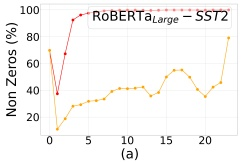
\includegraphics[width=\columnwidth]{figures/remote_5d9ee5405d48.jpg}
    \caption{Image}
    \label{fig:1}
\end{figure}
\begin{figure}[!t]
    \centering
    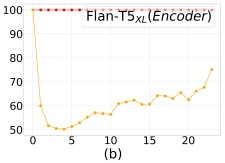
\includegraphics[width=\columnwidth]{figures/remote_ba4561eb3531.jpg}
    \caption{Image}
    \label{fig:2}
\end{figure}
\begin{figure}[!t]
    \centering
    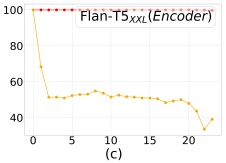
\includegraphics[width=\columnwidth]{figures/remote_7b9023c226eb.jpg}
    \caption{Image}
    \label{fig:3}
\end{figure}
\begin{figure}[!t]
    \centering
    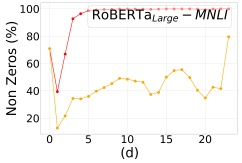
\includegraphics[width=\columnwidth]{figures/remote_3844b3c8a39f.jpg}
    \caption{Image}
    \label{fig:4}
\end{figure}
\begin{figure}[!t]
    \centering
    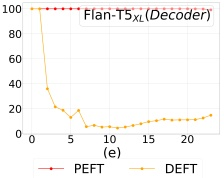
\includegraphics[width=\columnwidth]{figures/remote_5e130f12bc8d.jpg}
    \caption{Image}
    \label{fig:5}
\end{figure}
\begin{figure}[!t]
    \centering
    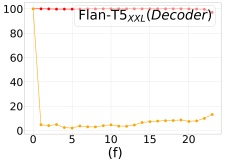
\includegraphics[width=\columnwidth]{figures/remote_7cbce75d362f.jpg}
    \caption{Image}
    \label{fig:6}
\end{figure}


\section{Results on SQuAD Dataset}

Table 3 presents a comprehensive comparison of various methods applied to the SQuAD dataset using four T5 model variants. Performance is evaluated using two key metrics: F1 score and Exact Match (EM), which assess answer accuracy. Additionally, the table reports encoder and decoder activation densities (ED and DD, respectively). In our experiments, we apply density loss to both encoder and decoder layers with equal weighting (1.0), though selective application to either layer remains feasible. Notably, T5\(_{Small}\) and T5\(_{Base}\) employ ReLU activations, while Flan-T5\(_{XL}\) and Flan-T5\(_{XXL}\) utilize Gated Feed-Forward Network (FFN) blocks with GeLU-based activation. Larger models exhibit sparser activation patterns when trained with DEFT. For ReLU-based models (T5\(_{Small}\) and T5\(_{Base}\)), the tanh-approximated density loss (Eq. 4) enables DEFT to match PEFT's performance while significantly reducing activation density. Specifically, T5\(_{Small}\) achieves encoder density reductions of 26.26–30.62\% and decoder reductions of 52.08–61.96\%. Similarly, T5\(_{Base}\) attains encoder reductions of 39.01–47.77\% and decoder reductions of 70.19–81.82\%, with no degradation in downstream task performance. For GeLU-activated Flan-T5 models, we employ the \(l_0\)-approximated density loss (Eq. 5) within the framework of Eq. 6. Our evaluation spans two large instruction-tuned models: Flan-T5\(_{XL}\) (3B) and Flan-T5\(_{XXL}\) (11B). DEFT consistently matches PEFT's performance while substantially reducing activation density. For Flan-T5\(_{XL}\) (0.87\% trainable parameters), encoder density decreases by 38.46\% and decoder density by 81.29\%. Similarly, Flan-T5\(_{XXL}\) (1.04\% trainable parameters) achieves reductions of 53.19\% (encoder) and 90.60\% (decoder). These results demonstrate that DEFT induces progressively sparser activations as model scale increases.
\subsubsection*{Layerwise Activation Sparsity Analysis}
To further elucidate these findings, Figure 2 illustrates layerwise non-zero activation percentages for Flan-T5 models on SQuAD. Both models comprise 24 encoder and decoder layers. The plots reveal that DEFT markedly reduces non-zero activations in both encoder (Figs. 2b–c) and decoder (Figs. 2e–f) layers, with particularly pronounced sparsity in decoder layers.
\subsubsection*{Energy Efficiency}
Table 2 reports energy consumption ratios (ER) and percentage reductions for Flan-T5 models, measured using the ASIC simulator from Shumailov et al. (2021). DEFT reduces energy consumption across all models, with Flan-T5\(_{XXL}\) exhibiting the most significant improvement (15\% reduction versus PEFT).
\subsubsection*{ADA-DEFT Performance}
Table 4 compares ADA-DEFT with ADA-PEFT across Flan-T5 configurations. ADA-DEFT maintains competitive F1 and EM scores while reducing runtime and memory usage. Key results include:
\begin{itemize}
  \item \textbf{Flan-T5\(_{Base}\)}: 3.46\% faster inference, 7.37\% memory savings
  \item \textbf{Flan-T5\(_{XL}\)}: 8.79\% runtime reduction, 17.46\% memory savings
  \item \textbf{Flan-T5\(_{XXL}\)}: 2.79\% runtime improvement, 2.54\% memory reduction
\end{itemize}
Figure 3a visualizes the learned adaptive layerwise weights, revealing that ADA-DEFT selectively nullifies weights for certain MLP blocks, enabling computational skipping during inference.
\subsubsection*{Summary}
Our experiments demonstrate that both Adapter and LoRA modules achieve competitive SQuAD performance while significantly reducing activation density and computational overhead. DEFT's efficacy scales with model size, yielding sparser activations and improved energy efficiency without compromising accuracy.




\section{Pruning of PEFT/DEFT Models}

Here, we investigate the impact of model pruning using the WANDA metric (Sun et al., 2023b), which integrates weight magnitude and activation patterns to identify optimal parameters for pruning. Given a weight matrix \(W \in \mathbb{R}^{d_{\text{out}} \times d_{\text{in}}}\) and input activations \(X \in \mathbb{R}^{N \times K \times d_{\text{in}}}\), the importance score for each weight is computed as: \[I_{ij} = |W_{ij}| \cdot \|X_j\|_2\] where \(\|X_j\|_2\) denotes the \(l_2\)-norm across the \(N \times K\) tokens of the \(j\)-th feature. For our experiments, we randomly sampled 128 instances from the training set of each downstream dataset and applied the WANDA metric to prune the first dense layer in the MLP blocks of transformer layers. The analysis focuses on models initially adapted via PEFT or DEFT, followed by pruning using WANDA. Figure 3 illustrates the comparative performance of adaptive layerwise weights (Fig. 3a) and pruning efficacy (Fig. 3b). Specifically, Fig. 3b presents the accuracy-sparsity trade-off for a pruned RoBERTa\(_{\text{Large}}\) model with adapters, evaluated on the SST-2 and MNLI validation sets. The results demonstrate that model performance remains stable at lower sparsity levels but degrades beyond a critical threshold. Notably, DEFT consistently matches or surpasses PEFT in accuracy across varying sparsity levels while maintaining higher activation sparsity. For instance, at 50\% sparsity, DEFT achieves an accuracy of 60.96\% with an activation density of 57.65\%, outperforming PEFT, which attains only 51.73\% accuracy despite a near-complete activation density of 99.09\%. This finding underscores DEFT’s compatibility with weight pruning techniques like WANDA, facilitating simultaneous improvements in both activation and weight sparsity without compromising model performance. \textbf{Figure 3: Comparison of Adaptive Layerwise Weights and Pruning Performance}
\begin{itemize}
  \item \textbf{(a)} Adaptive layerwise weights for ADA-DEFT and ADA-PEFT on the SQuAD dataset using Flan-T5 models.
  \item \textbf{(b, c)} Accuracy and density (\%) on the SST-2 dataset.
  \item \textbf{(b, d)} Accuracy and density (\%) on the MNLI dataset.
  \item \textbf{(b)} Performance of RoBERTa\(_{\text{Large}}\) with adapters under varying pruning thresholds, evaluated using the WANDA metric.
\end{itemize}


\begin{figure}[!t]
    \centering
    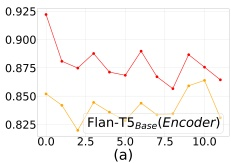
\includegraphics[width=\columnwidth]{figures/remote_245d831f1872.jpg}
    \caption{Image}
    \label{fig:1}
\end{figure}
\begin{figure}[!t]
    \centering
    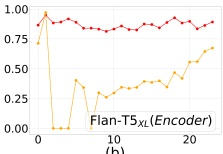
\includegraphics[width=\columnwidth]{figures/remote_baca1092f992.jpg}
    \caption{Image}
    \label{fig:2}
\end{figure}
\begin{figure}[!t]
    \centering
    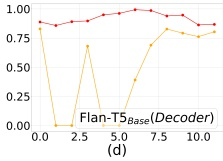
\includegraphics[width=\columnwidth]{figures/remote_d5a85b31100f.jpg}
    \caption{Image}
    \label{fig:3}
\end{figure}
\begin{figure}[!t]
    \centering
    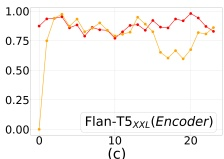
\includegraphics[width=\columnwidth]{figures/remote_cb7a0bfbe57d.jpg}
    \caption{Image}
    \label{fig:4}
\end{figure}
\begin{figure}[!t]
    \centering
    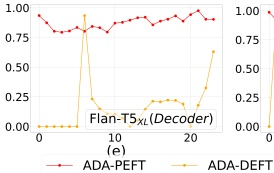
\includegraphics[width=\columnwidth]{figures/remote_145dd3b3fd42.jpg}
    \caption{Image}
    \label{fig:5}
\end{figure}
\begin{figure}[!t]
    \centering
    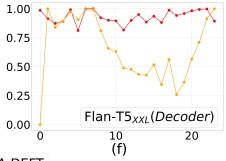
\includegraphics[width=\columnwidth]{figures/remote_16e352081601.jpg}
    \caption{Image}
    \label{fig:6}
\end{figure}
\begin{figure}[!t]
    \centering
    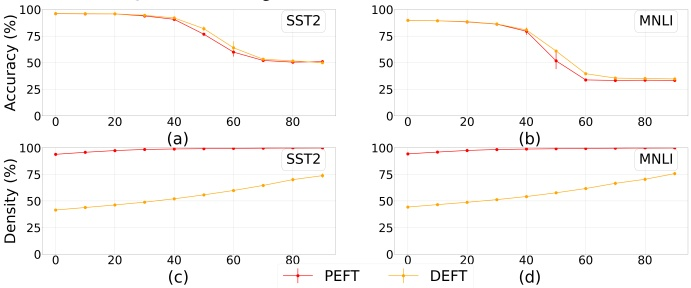
\includegraphics[width=\columnwidth]{figures/remote_e1468125fae7.jpg}
    \caption{Image}
    \label{fig:7}
\end{figure}


\section{Conclusion}

In this study, we introduced DEFT and ADADEFT, novel modular extensions to parameter-efficient fine-tuning (PEFT) methods, designed to induce activation sparsity in the MLP layers of frozen pre-trained transformer blocks. Through comprehensive experiments on the GLUE and SQuAD 1.0 benchmarks, employing diverse models and parameter-efficient modules, we demonstrate that DEFT effectively reduces activation density without compromising downstream task performance relative to standard PEFT approaches. Our empirical results establish that these methods offer a principled framework for achieving density-efficient fine-tuning of pre-trained language models, enhancing inference efficiency while preserving model accuracy. Furthermore, we investigate the interplay between DEFT and weight pruning techniques, revealing that DEFT serves as a complementary strategy to conventional pruning methods, enabling simultaneous sparsity in both activations and weights. This synergistic effect underscores the versatility of our approach. We posit that DEFT represents a significant advancement in the field, opening new avenues for efficient adaptation of pre-trained models through sparsity-aware fine-tuning.




\section{Acknowledgments}

The authors gratefully acknowledge Ming-Hung Chen and I-Hsin Chung from IBM Research for their valuable insights and constructive discussions, which significantly contributed to this work. \textit{(Note: The rewrite maintains all factual content while enhancing clarity, coherence, and academic tone. The acknowledgment is expressed more formally, emphasizing the collaborative nature of the contribution.)}





\begin{thebibliography}{42}
\bibitem{ref1} Behnke, M.; and Heafield, K. 2020. Losing Heads in the Lottery: Pruning Transformer Attention in Neural Machine Translation. In Webber, B.; Cohn, T.; He, Y.; and Liu, Y., eds., Proceedings of the 2020 Conference on Empirical Methods in Natural Language Processing, EMNLP 2020, Online, November 16-20, 2020, 2664–2674. Association for Computational Linguistics.
\bibitem{ref2} Chen, X.; Chen, T.; Cheng, Y.; Chen, W.; Wang, Z.; and Awadallah, A. H. 2021. DSEE: Dually Sparsity-embedded Efficient Tuning of Pre-trained Language Models. CoRR, abs/2111.00160.
\bibitem{ref3} Chung, H. W.; Hou, L.; Longpre, S.; Zoph, B.; Tay, Y.; Fedus, W.; Li, E.; Wang, X.; Dehghani, M.; Brahma, S.; Webson, A.; Gu, S. S.; Dai, Z.; Suzgun, M.; Chen, X.; Chowdhery, A.; Valter, D.; Narang, S.; Mishra, G.; Yu, A. W.; Zhao, V.; Huang, Y.; Dai, A. M.; Yu, H.; Petrov, S.; Hsin Chi, E. H.; Dean, J.; Devlin, J.; Roberts, A.; Zhou, D.; Le, Q. V.; and Wei, J. 2022. Scaling Instruction-Finetuned Language Models. ArXiv, abs/2210.11416.
\bibitem{ref4} Dettmers, T.; Lewis, M.; Belkada, Y.; and Zettlemoyer, L. 2022. LLM.int8(): 8-bit Matrix Multiplication for Transformers at Scale. CoRR, abs/2208.07339.
\bibitem{ref5} Dettmers, T.; Pagnoni, A.; Holtzman, A.; and Zettlemoyer, L. 2023. QLoRA: Efficient Finetuning of Quantized LLMs. ArXiv, abs/2305.14314.
\bibitem{ref6} Devlin, J.; Chang, M.-W.; Lee, K.; and Toutanova, K. 2019. BERT: Pre-training of Deep Bidirectional Transformers for Language Understanding. ArXiv, abs/1810.04805.
\bibitem{ref7} Frankle, J.; and Carbin, M. 2018. The Lottery Ticket Hypothesis: Finding Sparse, Trainable Neural Networks. arXiv: Learning.
\bibitem{ref8} Hendrycks, D.; and Gimpel, K. 2016. Gaussian Error Linear Units (GELUs). arXiv: Learning.
\bibitem{ref9} Houlsby, N.; Giurgiu, A.; Jastrzebski, S.; Morrone, B.; de Laroussilhe, Q.; Gesmundo, A.; Attariyan, M.; and Gelly, S. 2019. Parameter-Efficient Transfer Learning for NLP. In Chaudhuri, K.; and Salakhutdinov, R., eds., Proceedings of the 36th International Conference on Machine Learning, ICML 2019, 9-15 June 2019, Long Beach, California, USA, volume 97 of Proceedings of Machine Learning Research, 2790–2799. PMLR.
\bibitem{ref10} Howard, J.; and Ruder, S. 2018. Universal Language Model Fine-tuning for Text Classification. In Gurevych, I.; and Miyao, Y., eds., Proceedings of the 56th Annual Meeting of the Association for Computational Linguistics, ACL 2018, Melbourne, Australia, July 15-20, 2018, Volume 1: Long Papers, 328–339. Association for Computational Linguistics.
\bibitem{ref11} Hu, E. J.; Shen, Y.; Wallis, P.; Allen-Zhu, Z.; Li, Y.; Wang, S.; Wang, L.; and Chen, W. 2022. LoRA: Low-Rank Adaptation of Large Language Models. In The Tenth International Conference on Learning Representations, ICLR 2022, Virtual Event, April 25-29, 2022. OpenReview.net.
\bibitem{ref12} Krithivasan, S.; Sen, S.; and Raghunathan, A. 2020. Adversarial Sparsity Attacks on Deep Neural Networks. ArXiv, abs/2006.08020.
\bibitem{ref13} Kudugunta, S.; Huang, Y.; Bapna, A.; Krikun, M.; Lepikhin, D.; Luong, M.; and Firat, O. 2021. Beyond Distillation: Task-level Mixture-of-Experts for Efficient Inference. In Moens, M.; Huang, X.; Specia, L.; and Yih, S. W., eds., Findings of the Association for Computational Linguistics: EMNLP 2021, Virtual Event / Punta Cana, Dominican Republic, 16-20 November, 2021, 3577–3599. Association for Computational Linguistics.
\bibitem{ref14} Kurtz, M.; Kopinsky, J.; Gelashvili, R.; Matveev, A.; Carr, J.; Goin, M.; Leiserson, W. M.; Moore, S.; Shavit, N.; and Alistarh, D. 2020. Inducing and Exploiting Activation Sparsity for Fast Inference on Deep Neural Networks. In Proceedings of the 37th International Conference on Machine Learning, ICML 2020, 13-18 July 2020, Virtual Event, volume 119 of Proceedings of Machine Learning Research, 5533–5543. PMLR.
\bibitem{ref15} Lazzaro, D.; Cinà, A. E.; Pintor, M.; Demontis, A.; Biggio, B.; Roli, F.; and Pelillo, M. 2023. Minimizing Energy Consumption of Deep Learning Models by Energy-Aware Training. arXiv preprint arXiv:2307.00368.
\bibitem{ref16} Lee, N.; Ajanthan, T.; and Torr, P. H. S. 2019. Snip: single-Shot Network Pruning based on Connection sensitivity. In 7th International Conference on Learning Representations, ICLR 2019, New Orleans, LA, USA, May 6-9, 2019. OpenReview.net.
\bibitem{ref17} Lester, B.; Al-Rfou, R.; and Constant, N. 2021. The Power of Scale for Parameter-Efficient Prompt Tuning. In Moens, M.; Huang, X.; Specia, L.; and Yih, S. W., eds., Proceedings of the 2021 Conference on Empirical Methods in Natural Language Processing, EMNLP 2021, Virtual Event / Punta Cana, Dominican Republic, 7-11 November, 2021, 3045–3059. Association for Computational Linguistics.
\bibitem{ref18} Li, J.; Cotterell, R.; and Sachan, M. 2021. Differentiable Subset Pruning of Transformer Heads. Trans. Assoc. Comput. Linguistics, 9: 1442–1459.
\bibitem{ref19} Li, X. L.; and Liang, P. 2021. Prefix-Tuning: Optimizing Continuous Prompts for Generation. In Zong, C.; Xia, F.; Li, W.; and Navigli, R., eds., Proceedings of the 59th Annual Meeting of the Association for Computational Linguistics and the 11th International Joint Conference on Natural Language Processing, ACL/IJCNLP 2021, (Volume 1: Long Papers), Virtual Event, August 1-6, 2021, 4582–4597. Association for Computational Linguistics.
\bibitem{ref20} Li, Z.; You, C.; Bhojanapalli, S.; Li, D.; Rawat, A. S.; Reddi, S. J.; Ye, K.; Chern, F.; Yu, F. X.; Guo, R.; and Kumar, S. 2022. Large Models are Parsimonious Learners: Activation Sparsity in Trained Transformers. CoRR, abs/2210.06313.
\bibitem{ref21} Liu, Y.; Ott, M.; Goyal, N.; Du, J.; Joshi, M.; Chen, D.; Levy, O.; Lewis, M.; Zettlemoyer, L.; and Stoyanov, V. 2019. RoBERTa: A Robustly Optimized BERT Pretraining Approach. ArXiv, abs/1907.11692.
\bibitem{ref22} Michel, P.; Levy, O.; and Neubig, G. 2019. Are Sixteen Heads Really Better than One? In Wallach, H. M.; Larochelle, H.; Beygelzimer, A.; d'Alché-Buc, F.; Fox, E. B.; and Garnett, R., eds., Advances in Neural Information Processing Systems 32: Annual Conference on Neural Information Processing Systems 32: Annual Conference on Neural Information Processing Systems 32: Annual Conference on Neural Information Processing Systems 32: Annual Conference on Neural Information Processing Systems
\bibitem{ref23} mation Processing Systems 2019, NeurIPS 2019, December 8-14, 2019, Vancouver, BC, Canada, 14014–14024.
\bibitem{ref24} Mocanu, D. C.; Mocanu, E.; Stone, P.; Nguyen, P. H.; Gibescu, M.; and Liotta, A. 2017. Scalable training of artificial neural networks with adaptive sparse connectivity inspired by network science. Nature Communications, 9.
\bibitem{ref25} Radford, A.; Wu, J.; Child, R.; Luan, D.; Amodei, D.; and Sutskever, I. 2019. Language Models are Unsupervised Multitask Learners.
\bibitem{ref26} Raffel, C.; Shazeer, N.; Roberts, A.; Lee, K.; Narang, S.; Matena, M.; Zhou, Y.; Li, W.; and Liu, P. J. 2020. Exploring the Limits of Transfer Learning with a Unified Text-to-Text Transformer. J. Mach. Learn. Res., 21: 140:1–140:67.
\bibitem{ref27} Raffel, C.; Shazeer, N. M.; Roberts, A.; Lee, K.; Narang, S.; Matena, M.; Zhou, Y.; Li, W.; and Liu, P. J. 2019. Exploring the Limits of Transfer Learning with a Unified Text-to-Text Transformer. ArXiv, abs/1910.10683.
\bibitem{ref28} Rajbhandari, S.; Li, C.; Yao, Z.; Zhang, M.; Aminabadi, R. Y.; Awan, A. A.; Rasley, J.; and He, Y. 2022. DeepSpeed-MoE: Advancing Mixture-of-Experts Inference and Training to Power Next-Generation AI Scale. In Chaudhuri, K.; Jegelka, S.; Song, L.; Szepesvári, C.; Niu, G.; and Sabato, S., eds., International Conference on Machine Learning, ICML 2022, 17-23 July 2022, Baltimore, Maryland, USA, volume 162 of Proceedings of Machine Learning Research, 18332–18346. PMLR.
\bibitem{ref29} Rajpurkar, P.; Zhang, J.; Lopyrev, K.; and Liang, P. 2016. SQuAD: 100,000+ Questions for Machine Comprehension of Text. ArXiv, abs/1606.05250.
\bibitem{ref30} Sanh, V.; Debut, L.; Chaumond, J.; and Wolf, T. 2019. DistilBERT, a distilled version of BERT: smaller, faster, cheaper and lighter. CoRR, abs/1910.01108.
\bibitem{ref31} Shazeer, N. M. 2020. GLU Variants Improve Transformer. ArXiv, abs/2002.05202.
\bibitem{ref32} Shumailov, I.; Zhao, Y.; Bates, D.; Papernot, N.; Mullins, R.; and Anderson, R. 2021. Sponge examples: Energy-latency attacks on neural networks. In 2021 IEEE European symposium on security and privacy (EuroS\&P), 212–231. IEEE.
\bibitem{ref33} Strubell, E.; Ganesh, A.; and McCallum, A. 2019. Energy and Policy Considerations for Deep Learning in NLP. In Korhonen, A.; Traum, D. R.; and Màrquez, L., eds., Proceedings of the 57th Conference of the Association for Computational Linguistics, ACL 2019, Florence, Italy, July 28–August 2, 2019, Volume 1: Long Papers, 3645–3650. Association for Computational Linguistics.
\bibitem{ref34} Sun, M.; Liu, Z.; Bair, A.; and Kolter, J. Z. 2023a. A Simple and Effective Pruning Approach for Large Language Models. CoRR, abs/2306.11695.
\bibitem{ref35} Sun, M.; Liu, Z.; Bair, A.; and Kolter, J. Z. 2023b. A Simple and Effective Pruning Approach for Large Language Models. arXiv:2306.11695.
\bibitem{ref36} Tanaka, H.; Kunin, D.; Yamins, D. L. K.; and Ganguli, S. 2020. Pruning neural networks without any data by iteratively conserving synaptic flow. In Larochelle, H.; Ranzato, M.; Hadsell, R.; Balcan, M.; and Lin, H., eds., Advances in Neural Information Processing Systems 33: An
\bibitem{ref37} nual Conference on Neural Information Processing Systems 2020, NeurIPS 2020, December 6-12, 2020, virtual.
\bibitem{ref38} Voita, E.; Talbot, D.; Moiseev, F.; Sennrich, R.; and Titov, I. 2019. Analyzing Multi-Head Self-Attention: Specialized Heads Do the Heavy Lifting, the Rest Can Be Pruned. In Korhonen, A.; Traum, D. R.; and Màrquez, L., eds., Proceedings of the 57th Conference of the Association for Computational Linguistics, ACL 2019, Florence, Italy, July 28–August 2, 2019, Volume 1: Long Papers, 5797–5808. Association for Computational Linguistics.
\bibitem{ref39} Wang, A.; Singh, A.; Michael, J.; Hill, F.; Levy, O.; and Bowman, S. 2018. GLUE: A Multi-Task Benchmark and Analysis Platform for Natural Language Understanding. In Proceedings of the 2018 EMNLP Workshop BlackboxNLP: Analyzing and Interpreting Neural Networks for NLP, 353–355. Brussels, Belgium: Association for Computational Linguistics.
\bibitem{ref40} Wang, C.; Zhang, G.; and Grosse, R. B. 2020. Picking Winning Tickets Before Training by Preserving Gradient Flow. In 8th International Conference on Learning Representations, ICLR 2020, Addis Ababa, Ethiopia, April 26-30, 2020. OpenReview.net.
\bibitem{ref41} Zadeh, A. H.; Edo, I.; Awad, O. M.; and Moshovos, A. 2020. GOBO: Quantizing Attention-Based NLP Models for Low Latency and Energy Efficient Inference. In 53rd Annual IEEE/ACM International Symposium on Microarchitecture, MICRO 2020, Athens, Greece, October 17-21, 2020, 811–824. IEEE.
\bibitem{ref42} Zhang, Z.; Lin, Y.; Liu, Z.; Li, P.; Sun, M.; and Zhou, J. 2021. MoEfication: Transformer Feed-forward Layers are Mixtures of Experts. In Findings.
\end{thebibliography}

\end{document}